\subsection{Impacto das variáveis sobre o consumo anual de energia elétrica}
\noindent A etapa de otimização possibilitou visualizar a influência das variáveis sobre o consumo anual final das edificações para cada cenário definido. Os resultados da implementação das medidas ativas de redução de consumo de energia, disponíveis nos Apêndices deste trabalho, demonstraram maior peso entre as variáveis de estratégia ativa, pertencentes aos blocos de simulação 2, 3 e 9, e passivas, formadas pelos blocos de simulação 1, e de 4 a 10, como exposto nos Gráficos 4 e 5.\vspace*{0.3cm} \newline
\noindent Nota-se que as variáveis de estratégias ativas reduziram significativamente o consumo anual, com curvas de queda expressivas, direcionando a média de consumo para baixo, posicionando alguns cenários abaixo da média linear, como observado entre os blocos de simulação 1 ao 7 do Gráfico 4. Este comportamento se estende até o bloco de simulação 7 no modelo de 19 pavimentos, desempenho demonstrado no Gráfico 5. Os blocos de simulação compostos por variáveis passivas apresentaram constância de forma e estreitamento ao longo do avanço das implementações das medidas. O estreitamento gradativo da amplitude da curva de consumo final anual em ambos os resultados sugere que o avanço cumulativo das medidas de mitigação de consumo é importante para o sucesso do processo de adequação da edificação ao conceito \textit{Zero Energy}.\vspace*{0.3cm} \newline
\noindent A tendência ascendente das curvas de consumo, a partir do bloco de simulação 4, é causada pela alteração do PAF\textsubscript{T}, partindo da menor razão, de 30\%, até alcançar a maior razão entre área de fachada e área de aberturas envidraçadas, com 80\%. Esta medida aponta a importância da adoção de aberturas menores, em torno de 30\%, para a melhor relação entre o PAF\textsubscript{T} e o consumo energético da edificação.\vspace*{0.3cm} \newline
\noindent Os gráficos serviram como instrumento de tomada de decisão acerca da seleção dos melhores cenários para a etapa de simulação de geração de energia solar fotovoltaica. Além disso, os gráficos facilitaram a visualização da importância de cada estratégia adotada para o balanço energético nulo das edificações avaliadas. A leitura dos gráficos pode ser feita da seguinte forma:
\begin{itemize}
    \item Os gráficos consistem em evidenciar o impacto das medidas adotadas no consumo da edificação. Para tal, foi definida a comparação entre o desempenho dos modelos por meio do percentual de redução de consumo de energia entre as edificações. Esta comparação desconsidera a escala dos gráficos, já que ambos correspondem a edificações de portes diferentes, e considera o comportamento das medidas aplicadas por meio de análise das curvas de consumo;
    \item Os pontos na cor laranja representam cada cenário montado, os quais variam entre 4 conjuntos de implementação sequencial de medidas de redução de energia. Cada conjunto de cenários pertencentes aos 10 blocos de simulação estão definidos e representados nos Gráficos 4 e 5;
    \item As curvas em verde representam a tendência de aumento ou redução de consumo de 
    energia entre a simulação dos cenários;
    \item Como a mudança entre os tipos de vidro avaliados, foi necessário realizar novas simulações de todos os blocos anteriores a esta medida, sendo essa etapa representada pelas curvas acentuadas entre conjuntos de cenários, como, por exemplo, observado na curva entre os cenários 12 e 13 do bloco de simulação 10, na página 93.            
\end{itemize}
\noindent A redução de consumo provocada pela implementação de equipamentos e iluminação mais eficientes atinge o patamar de 22,48\% de redução global, assim como o sistema de arrefecimento, com 34,78\% para o modelo de 19 pavimentos. As reduções no modelo de 8 pavimentos foram tênues, da ordem de 16,09 e 16,66\%, respectivamente, para os sistemas de arrefecimento, e equipamentos e iluminação, como observado na Figura 21.\vspace*{0.3cm} \newline
\noindent Entretanto, cabe mencionar que o desempenho de controle térmico do sistema Split para o modelo de 19 pavimentos, nos cenários iniciais, provocou maior consumo de energia em relação aos dois outros sistemas de arrefecimento avaliados, CAG e VRF, em 22,73\%. Após a implementação do vidro mais eficiente, houve redução do consumo em cerca de 24,91\%, superando ligeiramente em performance o sistema CAG. Em contraste a esta observação do Split para o modelo de 19 pavimentos, este sistema obteve comportamento semelhante ao sistema VRF para a edificação de 8 pavimentos, com considerável performance e redução de consumo de energia. O \textit{Split} apresentou controle satisfatório das médias de temperatura de conforto das zonas térmicas. A diferença de desempenho dos sistemas de condicionamento de ar entre os dois modelos pode ser atribuída a diferença de carga térmica entre as edificações, onde o modelo de 8 pavimentos apresenta menor carga térmica e menor exposição à radiação solar em comparação ao modelo de 19 pavimentos.\vspace*{0.3cm} \newline
\begin{figure}[H]
    \centering
    \rotatebox{90}{
        \begin{minipage}{\textheight}
            \caption{Consumo \textit{versus} medidas do modelo genérico de 8 pavimentos.}
            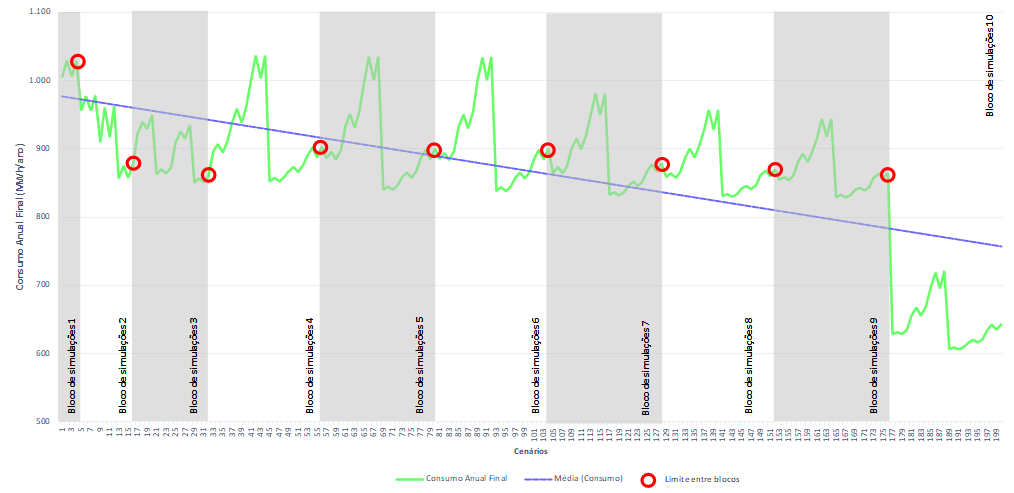
\includegraphics[width=1.0\textwidth]{figures/result/fig23-grafico4.png}
            \begin{flushleft}
                \par \small Fonte: autor, (2020). Legenda: Bloco de simulações 1 a 3 – Blocos com implementação do vidro, orientações solares e sistemas de condicionamento de ar; Bloco de simulações 4 –Bloco com implementação das variações de PAF\textsubscript{T}; Bloco de simulações 5 e 6 – Blocos com implementação de paredes e coberturas; Bloco de simulações 7 e 8 e 9 – Blocos com implementação das proteções solares; Bloco de simulações 10 – Blocos com implementação das medidas de redução de carga.
            \end{flushleft}
            \label{fig:figure23}
        \end{minipage}
    }
\end{figure}
\pagebreak

\begin{figure}[H]
    \centering
    \rotatebox{90}{
        \begin{minipage}{\textheight}
            \caption{Consumo \textit{versus} medidas do modelo genérico de 19 pavimentos.}
            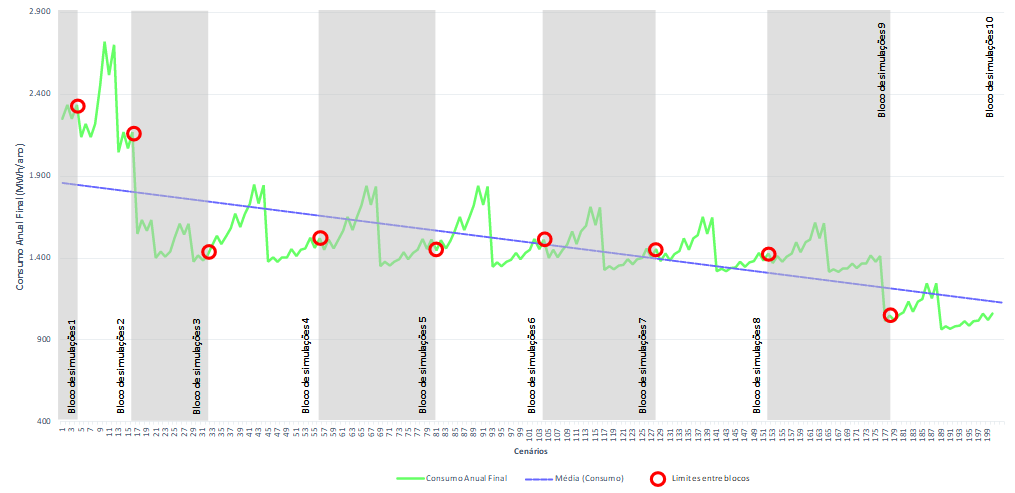
\includegraphics[width=1.0\textwidth]{figures/result/fig24-grafico5.png}
            \begin{flushleft}
                \par \small Fonte: autor, (2020). Legenda: Bloco de simulações 1 a 3 – Blocos com implementação do vidro, orientações solares e sistemas de condicionamento de ar; Bloco de simulações 4 –Bloco com implementação das variações de PAF\textsubscript{T}; Bloco de simulações 5 e 6 – Blocos com implementação de paredes e coberturas; Bloco de simulações 7 e 8 e 9 – Blocos com implementação das proteções solares; Bloco de simulações 10 – Blocos com implementação das medidas de redução de carga.
            \end{flushleft}
            \label{fig:figure24}
        \end{minipage}
    }
\end{figure}
\pagebreak
\noindent Como os vidros foram utilizados em todos os cenários, a importância da variável se torna mais visível quando comparado com todas as variáveis, assim como apresentado na Figura \ref{fig:figure25}. Verifica-se que, ao longo das implementações de medidas passivas, a influência é reduzida de 14,40\% para 4,00\%, conforme observado anteriormente nos blocos de simulação 3 e 4.\vspace*{0.3cm} \newline
\noindent Em ambos os resultados foi notado que a implementação de componentes construtivos com menor transmitância térmica acentua a diferença os cenários entre os modelos otimizados e os não-otimizados. Estes resultados retratam a importância das estratégias ativas para a redução do consumo total anual.
\begin{figure}[H]
    \centering
    \caption{Gráfico dos blocos de simulação das variáveis de vidro, orientação solar e do sistemas de condicionamento de ar e medidas de redução de carga dos modelos genérico de 8 (esq.) e 19 pavimentos (dir.)}
    \begin{subfigure}[b]{0.49\textwidth}
        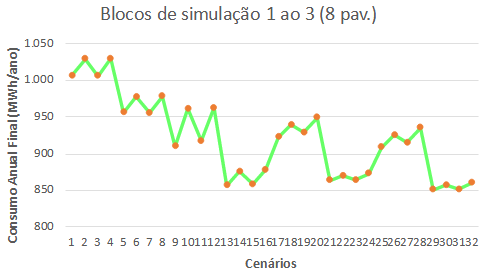
\includegraphics[width=\textwidth]{figures/result/fig25-bloco1-3.png}
    \end{subfigure}
    \begin{subfigure}[b]{0.49\textwidth}
        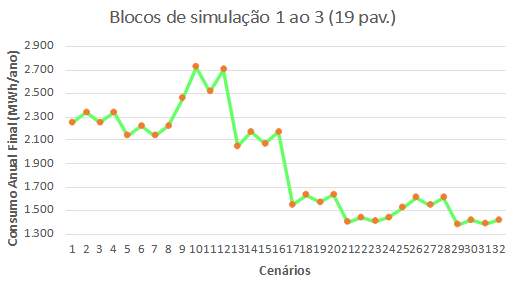
\includegraphics[width=\textwidth]{figures/result/fig26-bloco1-3.png}
    \end{subfigure}
    \begin{subfigure}[b]{0.49\textwidth}
        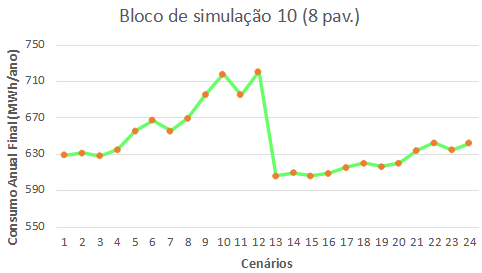
\includegraphics[width=\textwidth]{figures/result/fig27-bloco10.png}
    \end{subfigure}
    \begin{subfigure}[b]{0.49\textwidth}
        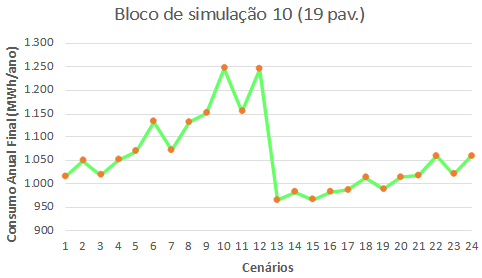
\includegraphics[width=\textwidth]{figures/result/fig28-bloco10.png}
    \end{subfigure}
    \begin{flushleft}
        \par \small Fonte: autor, (2020).
    \end{flushleft}
    \label{fig:figure25}
\end{figure}
\noindent As características das paredes e cobertura, blocos de simulação 5 e 6 respectivamente, na Figura 22, quando observadas isoladamente, são medidas importantes na redução de consumo, que neste caso representam 20\%, entre os componentes construtivos observados in loco e os componentes mais eficientes propostos para comparação. É verificada a suavização da curva de consumo entre o segundo conjunto de simulações, retratado pelos cenários 13 a 24, em relação ao primeiro conjunto, de 1 a 12, o que sinaliza a importância da envoltória e da redução da ação da radiação solar sobre os ambientes internos da edificação. A escala de consumo entre as edificações é acentuada nestes cenários, dada a semelhança do comportamento das curvas, porém, com amplitudes de 50 MW para o modelo de 8 pavimentos, e quase 200 MW para o modelo de 19 pavimentos.\vspace*{0.3cm} \newline
\noindent A influência destes componentes sobre o consumo final, junto ao vidro com baixa emissividade, atinge  o  patamar  de  26,72\%  para  a  análise  do  resultado  isolado,  como  exposto  na  Figura  \ref{fig:figure26}. Verifica-se, também, que as mudanças provocadas pela implementação das estratégias passivas, ao  longo  do  processo  de  otimização,  reduzem  a  relevância  do  vidro  com  menor  transmitância térmica para a composição construtiva e performance energética dos modelos.
\begin{figure}[H]
    \centering
    \caption{Gráficos dos blocos de simulação de paredes, 3, e coberturas, 4, dos modelos genéricos de 8 (esq.) e 19 pavimentos (dir.).}
    \begin{subfigure}[b]{0.49\textwidth}
        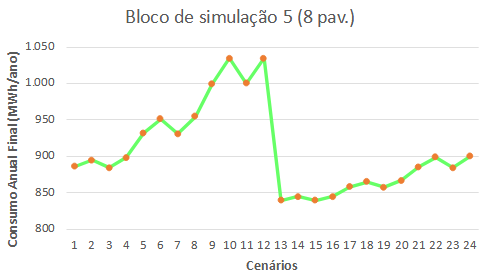
\includegraphics[width=\textwidth]{figures/result/fig29-bloco5.png}
    \end{subfigure}
    \begin{subfigure}[b]{0.49\textwidth}
        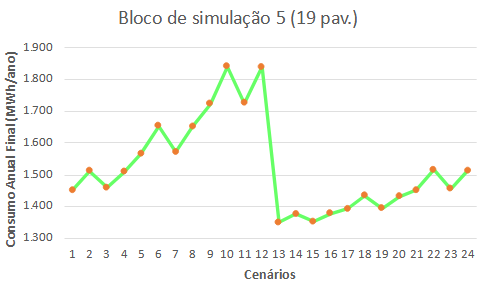
\includegraphics[width=\textwidth]{figures/result/fig30-bloco5.png}
    \end{subfigure}
    \begin{subfigure}[b]{0.49\textwidth}
        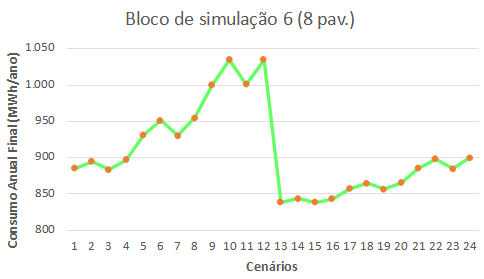
\includegraphics[width=\textwidth]{figures/result/fig31-bloco6.png}
    \end{subfigure}
    \begin{subfigure}[b]{0.49\textwidth}
        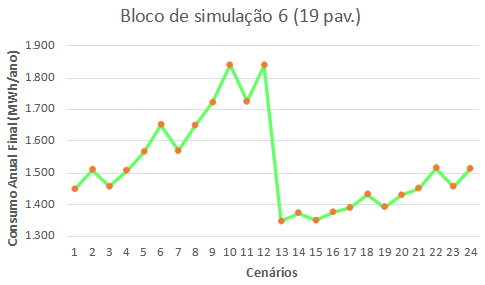
\includegraphics[width=\textwidth]{figures/result/fig32-bloco6.png}
    \end{subfigure}
    \begin{flushleft}
        \par \small Fonte: autor, (2020).
    \end{flushleft}
    \label{fig:figure26}
\end{figure}
\noindent As alterações sobre as variáveis do Percentual de Área de Abertura da Fachada Total, presentes na Figura \ref{fig:figure27}, representaram pouco impacto sobre o consumo final total quando comparado com as outras medidas implementadas. Entretanto, cabe citar que esta variável, quando observada isoladamente, corresponde a mesma grandeza de redução de consumo que as variáveis de componentes construtivos, reduzindo o consumo nos cenários simulados em cerca 18,95\% e 26,71\% para as edificações de 8 e 19 pavimentos, respectivamente. 
\begin{figure}[H]
    \centering
    \caption{Gráficos dos blocos de simulação de PAF\textsubscript{T} dos modelos genérico de 8 (esq.) e 19 pavimentos (dir.).}
    \begin{subfigure}[b]{0.49\textwidth}
        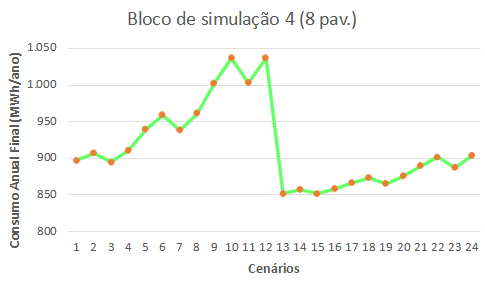
\includegraphics[width=\textwidth]{figures/result/fig33-bloco4.png}
    \end{subfigure}
    \begin{subfigure}[b]{0.49\textwidth}
        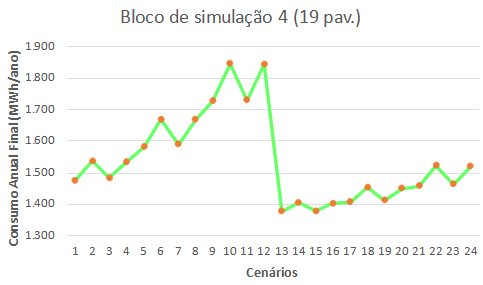
\includegraphics[width=\textwidth]{figures/result/fig34-bloco4.png}
    \end{subfigure}
    \begin{flushleft}
        \par \small Fonte: autor, (2020).
    \end{flushleft}
    \label{fig:figure27}
\end{figure}
A implementação das proteções solares, Figura \ref{fig:figure28}, apresentou redução de 6,96\% sobre o consumo total entre os blocos de simulação 5 e 6. Além desta redução, nota-se o estreitamento entre os cenários 12 e 13 neste bloco, em 23,52\%, reduzindo em 3,19\% a em relação aos blocos anteriores. Nota-se também a suavização da curva nos cenários 13 a 24 em ambas as simulações do modelo de 8 pavimentos, o que sugere a influência sobre o consumo ao controlar a quantidade de luz e de radiação no ambiente, por meio da implantação de proteções solares e de vidros mais eficientes.
\begin{figure}[H]
    \centering
    \caption{Bloco de simulações de protetores solares dos modelos genérico de 8 (esq.) e 19 pavimentos (dir.).}
    \begin{subfigure}[b]{0.49\textwidth}
        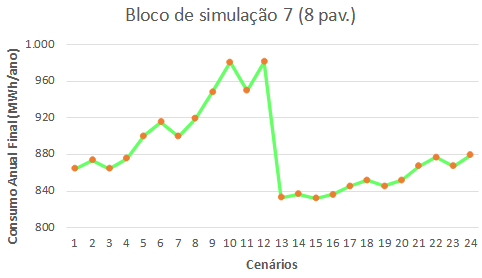
\includegraphics[width=\textwidth]{figures/result/fig35-bloco7.png}
    \end{subfigure}
    \begin{subfigure}[b]{0.49\textwidth}
        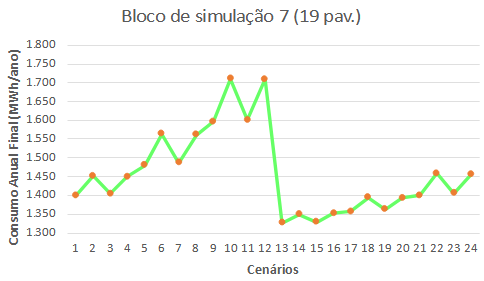
\includegraphics[width=\textwidth]{figures/result/fig36-bloco7.png}
    \end{subfigure}
    \begin{subfigure}[b]{0.49\textwidth}
        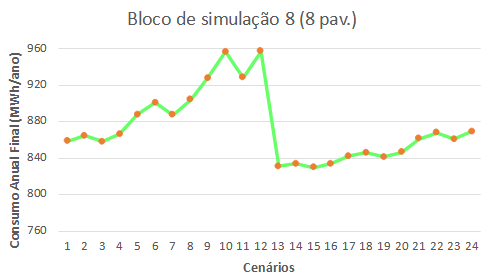
\includegraphics[width=\textwidth]{figures/result/fig37-bloco8.png}
    \end{subfigure}
    \begin{subfigure}[b]{0.49\textwidth}
        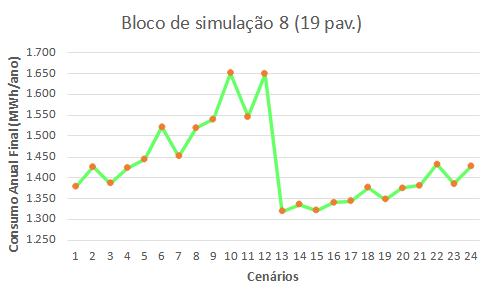
\includegraphics[width=\textwidth]{figures/result/fig38-bloco8.png}
    \end{subfigure}
    \begin{subfigure}[b]{0.49\textwidth}
        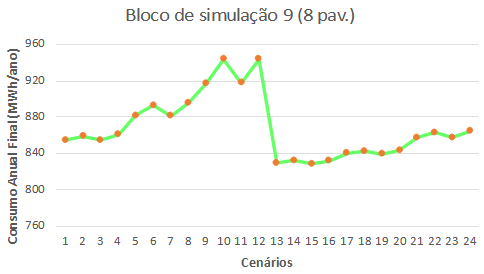
\includegraphics[width=\textwidth]{figures/result/fig39-bloco9.png}
    \end{subfigure}
    \begin{subfigure}[b]{0.49\textwidth}
        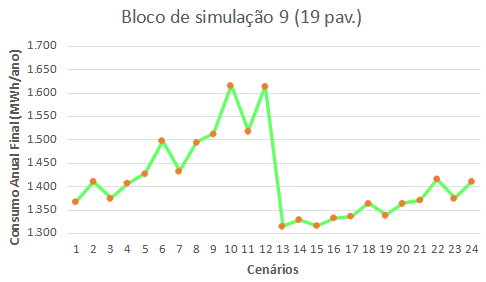
\includegraphics[width=\textwidth]{figures/result/fig40-bloco9.png}
    \end{subfigure}
    \begin{flushleft}
        \par \small Fonte: autor, (2020).
    \end{flushleft}
    \label{fig:figure28}
\end{figure}